%!TEX root = main.tex

Here we first give an overview and formalization of our model, 
and then describe its components.

\subsection{Formalization}

We assume both the premise tree and the hypothesis tree are 
binarized.

We use the premise tree and hypothesis tree 
in Figure~\ref{fig:egtree} to demonstrate the process 
of our approach.
The premise sentence is ``two women are hugging one another'',
and the hypothesis sentence is ``the women are sleeping''.

Following the traditional approaches \cite{maccartney2009extended,watanabe2012latent}, 
we first find the alignments from hypothesis
tree nodes to premise tree nodes
(i.e., the dashed or dotted curves in Figure~\ref{fig:egtree}).
Then we explore inducing the sentence-level 
entailment relations by 
1) first computing the entailment relation
at each node of the hypothesis tree based on the alignments, 
and then 2) composing the entailment relations
at the internal hypothesis nodes from bottom up
to the root in a recursive way.
Our model resembles the work of Natural Logic
\cite{maccartney2009extended} in the spirit 
that the entailment relation is inferred {\it modularly},
and composed {\it recursively}.

We formalize this entailment task as a structured prediction problem
similar to \newcite{mnih2014recurrent}, \newcite{ba2015learning}, and \newcite{xu2015show}.
The inputs are two trees: premise tree $P$,
and hypothesis tree $Q$. The goal is to predict a label
$y \in \{\text{contradiction}, \text{neutral}, \text{entailment}\}$.
Note that although the output label $y$ is not structured,
we can still consider the problem as a structured prediction problem,
because: 1) the input is a pair of trees; and 2)
the internal alignments are structured.

More formally, we aim to minimize the negative 
log likelihood of the 
gold label given the two trees. The objective
can be written in the online fashion as:
\vspace{-0.2cm}
\begin{align*}
\ell = & -\log\Prob(y|P, Q) = -\log \sum_{\mtxa} \Prob(y, \mtxa|P, Q)\\
= & -\log \sum_{\mtxa} \Prob(\mtxa|P, Q)\cdot \Prob(y|\mtxa, P, Q)
=  -\log \expect_{\Prob(\mtxa|P, Q)} [\Prob(y|\mtxa, P, Q)],
\end{align*}\\[-0.5cm]
where the structured latent variable
$\mtxa\in \{0, 1\}^{|Q|\times |P|}$ represents an alignment.
$\card{\cdot}$ is the number of nodes in the tree.
$\mtxa_{ij}=1$ if and only if node $i$ in $Q$ is aligned to node $j$
in $P$, otherwise $\mtxa_{ij}=0$.

%Our structured entailment model accomplish these two objectives
%in one step of calculation 
%and will be discussed in Section~\ref{sec:entailment}.

However, enumerating over all possible alignments $\mtxa$ takes exponential
time, we need to efficiently approximate the above log expectation.

Fortunately, as \newcite{xu2015show} point out, as long as the calculation
$\Prob(y|\mtxa, P, Q)$ only consists of linear calculation,
simple nonlinearities like $\tanh$, and softmax, we can 
have following simplification via first-order Taylor
approximation:
%\begin{align*}
\[
\ell =  -\log \expect_{\Prob(\mtxa|P, Q)} [\Prob(y|\mtxa, P, Q)]
\approx  -\log \Prob(y|\expect_{\Prob(\mtxa|P, Q)}[\mtxa], P, Q)],
%\end{align*}
\]\\[-0.7cm]
which means instead of enumerating over all alignments 
and calculating the label probability for each alignment,
we can use the label probability for the expected alignment 
as an approximation:\footnote{
We use bold letter, $\mtxa$,
for binary alignments, and tilde version, $\tilde{\mtxa}$, for the 
expected alignments in the real number space.
}
\begin{equation}
\tilde{\mtxa} \defeq \expect_{\Prob(\mtxa|P, Q)}[\mtxa] \quad \in \mathbb{R}^{\card{Q}\times \card{P}}
\label{eq:expatt}
\end{equation}\\[-0.7cm]
Figure~\ref{fig:exptalign} shows an example of expected
alignment calculation.
The objective is simplified to
\begin{equation}
\ell \approx -\log \Prob(y|\tilde{\mtxa}, P, Q).
\label{eq:newobj}
\end{equation}\\[-1.1cm]


\captionsetup[subfigure]{position=b}
\begin{figure*}
\raisebox{1.02in}{
\begin{subfigure}[t]{0.48\textwidth}
%\begin{center}
$\quad\ \ \ \frac{1}{3}\cdot$\raisebox{-.5\height}{
\includegraphics[width=0.2\textwidth]{avgalign.0.pdf}}
$\quad+\quad \frac{1}{2}\cdot$\raisebox{-.5\height}{
\includegraphics[width=0.2\textwidth]{avgalign.1.pdf}}\\[0.1in]
$\quad+\quad \frac{1}{6}\cdot$\raisebox{-.5\height}{
\includegraphics[width=0.2\textwidth]{avgalign.2.pdf}}
$\quad=\quad\ \ \  $\raisebox{-.5\height}{
\includegraphics[width=0.2\textwidth]{avgalign.3.pdf}}
%\end{center}
\caption{Expected alignment over 3 alignments with probability distribution of $(\frac{1}{3}, \frac{1}{2}, \frac{1}{6})$.
Each alignment is a matrix of $\{0, 1\}^{4\times 4}$,
and the expected alignment is a matrix of $\mathbb{R}^{4\times 4}$.
\label{fig:exptalign}}
\end{subfigure}
}
$\ $
\begin{subfigure}[t]{0.48\textwidth}
%\begin{center}
\includegraphics[width=0.9\textwidth]{arch}
%\end{center}
\caption{Architecture of our neural network.
Layers with the same color share the same parameters.
%In this network, first the Binary-Tree LSTM
%computes the meaning representations for each
%tree node. Then the Alignment module
The alignment module
calculates the expected alignment $\tilde{\mtxa}$.
%based on the node meaning representation.
The Entailment Composition module
infers the final entailment $y$.%relation along the 
%hypothesis tree from bottom up
%using the node meaning representation
%and the expected alignment.
\label{fig:arch}}
\end{subfigure}
\vspace{-0.2cm}
\caption{Expected alignments calculation (a) and overview of the network architecture (b).}
\vspace{-0.5cm}
\end{figure*}

With this observation, we split our calculation into two steps
as the top two modules in Figure~\ref{fig:arch}.
First in the Alignment module,
we calculate the expected alignments 
$\tilde{\mtxa}$ using Equation~\ref{eq:expatt} 
(Section~\ref{sec:att}).
Then we calculate the node-wise
entailment relation, propagate and compose the relation from
bottom up to find out the final entailment relation 
(Equation~\ref{eq:newobj})
in the Entailment Composition module
(Section~\ref{sec:ent}).
Both of these two modules rely on the composition of tree node meaning
representations (Section~\ref{sec:treelstm}).

\iffalse
\begin{figure}
\vspace{-0.4cm}
\begin{center}
\includegraphics[width=0.48\textwidth]{figures/arch}
\end{center}
\caption{Architecture of our neural network.
Layers with the same color share the same parameters.
In this network, first the Binary-Tree LSTM
computes the meaning representations for each
tree node. Then the Alignment module
calculates the expected alignment
based on the node meaning representation.
Finally the Entailment Composition module
infers the entailment relation along the 
hypothesis tree from bottom up
using the node meaning representation
and the expected alignment.
\label{fig:arch}}
%\vspace{-0.4cm}
\end{figure}
\fi

%%%%%%%%%%%%%%%%%%%%%%%%%%%%%%%%%%%%%%%%%%%%%%%%%%%%%%
\subsection{Attention over Tree Nodes}
\label{sec:att}
First we calculate the expected alignments
 $\tilde{\mtxa}$ between the hypothesis $Q$ and the premise $P$ (Equation~\ref{eq:expatt}):
\[\tilde{\mtxa} = \expect_{\Prob(\mtxa|P, Q)}[\mtxa].\]

To simplify the calculation, we further
approximate the global (binary) alignment $\mtxa$
to be consisted of the alignment 
$\mtxa_i \in \{0, 1\}^{1\times |P|}$ 
of each tree node $i\in Q$
independently. $\mtxa_i$ is the $i$th row of $\mtxa$:
\[\mtxa = [\mtxa_1^T;\mtxa_2^T;\dots;\mtxa_{\card{Q}}^T]^T,\]\vspace{-0.2in}
\[\Prob(\mtxa|P, Q) = \prod_i^{\card{Q}} \Prob(\mtxa_i|P, Q).\]
$\Prob(\mtxa_{i,j}=1|P, Q)$ is the probability 
of the node $i\in Q$ being aligned to node $j\in P$,
which is defined as:
\begin{equation}
\Prob(\mtxa_{i,j}=1|P, Q) \defeq 
\frac{\exp(T_{2k, 1}([\vech_i;\vech_j]))}{\sum_k\exp(T_{2k, 1}([\vech_i;\vech_k]))}.\label{eq:att}
\end{equation}
$\vech_i, \vech_j \in \mathbb{R}^k$ are vectors representing the semantic meanings of node $i$, $j$, respectively,
whose calculation will be described in Section~\ref{sec:treelstm}.
$T_{2k,1}$ is an affine transformation 
from $\mathbb{R}^{2k}$ to $\mathbb{R}$.
This formulation essentially is equivalent to 
the widely used attention
calculation in neural networks \cite{bahdanau2014neural}, i.e.,
for each node $i\in Q$, we find the relevant 
nodes $j\in P$ and use the softmax of the relevances 
as a probability distribution. In the rest of the paper,
we use ``expected alignment'' and ``attention'' interchangeably.

The expected alignment of node $i$ being aligned to node $j$, 
by definition, is:
\[
\tilde{\mtxa}_{i,j} = \Prob(\mtxa_{i,j}=1|P,Q) \cdot 1 = \Prob(\mtxa_{i,j}=1|P,Q).
\]
%Similarly we use $\tilde{\mtxa}_{i,j}$ to denote the probability 
%that node $i$ being aligned to node $j$:
%\[
%\tilde{\mtxa}_{i,j} = \sum_{\mtxa_i} \Prob(\mtxa_i|P, Q) \mtxa_i\quad \in \mathbb{R}^{1\times\card{P}}.
%\]

%%%%%%%%%%%%%%%%%%%%%%%%%%%%%%%%%%%%%%%%%%%%%%%%%%%%%%
\subsection{Entailment Composition}
\label{sec:ent}

Now we can calculate the entailment relation at each tree node
and propagate the entailment relation following
the hypothesis tree from bottom up, assuming the expected alignment
is given (Equation~\ref{eq:newobj}):
\[\ell \approx -\log \Prob(y|\tilde{\mtxa}, P, Q).
\]

Let vector $\vece_i \in \mathbb{R}^r$ denote the entailment relation in a 
latent relation space
at hypothesis tree node $i\in Q$. 
At the root of the hypothesis tree.
We can induce the final entailment relation from entailment relation vector
 $\vece_{\text{root}}$. We use a simple $\tanh$ layer
to project the entailment relation to the 3 relations
defined in the task, and use a softmax layer to 
calculate the probability for each relation:
\[
\Prob(y|\tilde{\mtxa}, P, Q) = \text{softmax}(\tanh (T_{r, 3}( \vece_{\text{root}}))).
\]

At each hypothesis node $i$, $\vece_i$ is calculated recursively given
the meaning representation at this tree node $\vech_i$,
the meaning representation of every node in the premise tree $\vech_j, j\in P$,
and the entailment from $i$'s children, $\vece_{i, 1}, \vece_{i, 2}$:
\begin{equation}
\vece_i 
= f_{\text{rel}}([\vech_i; \sum_{j\in P}\tilde{\mtxa}_{i,j} \vech_j], \vece_{i, 1}, \vece_{i, 2})
\label{eq:relcomp}
\end{equation}


\iffalse
Note the resemblance between the above function
and the definition of Binary-Tree LSTM transition function
(Equation~\ref{eq:lstmdef}),
this suggests that we can directly use a Binary-Tree LSTM
layer to calculate the entailment 
in a way similar to \newcite{wang2015learning}.
That is, using $[\vech_i; \sum_{j\in P}\mtxa_{i,j} \vech_j]$
as the input, and $\vece_{i, 1}$, $\vece_{i, 2}$ as 
the hidden states passed from children.\footnote{
We also need to add two vectors representing the memories
from the children.
}
\fi
Figure~\ref{fig:entnode} illustrates the calculation
of the entailment composition.
%We have various choices for the composition function $f(\cdot)$
%in Equation~\ref{eq:relcomp}.
We will discuss $f_{\text{rel}}$ in Section~\ref{sec:treelstm}.

%%%%%%%%%%%%%%%%%%%%%%%%%%%%%%%%%%%%%%%%%%%%%%%%%%%%%%

\begin{figure}
%\begin{center}
\centering
\begin{subfigure}[b]{0.49\textwidth}
\centering
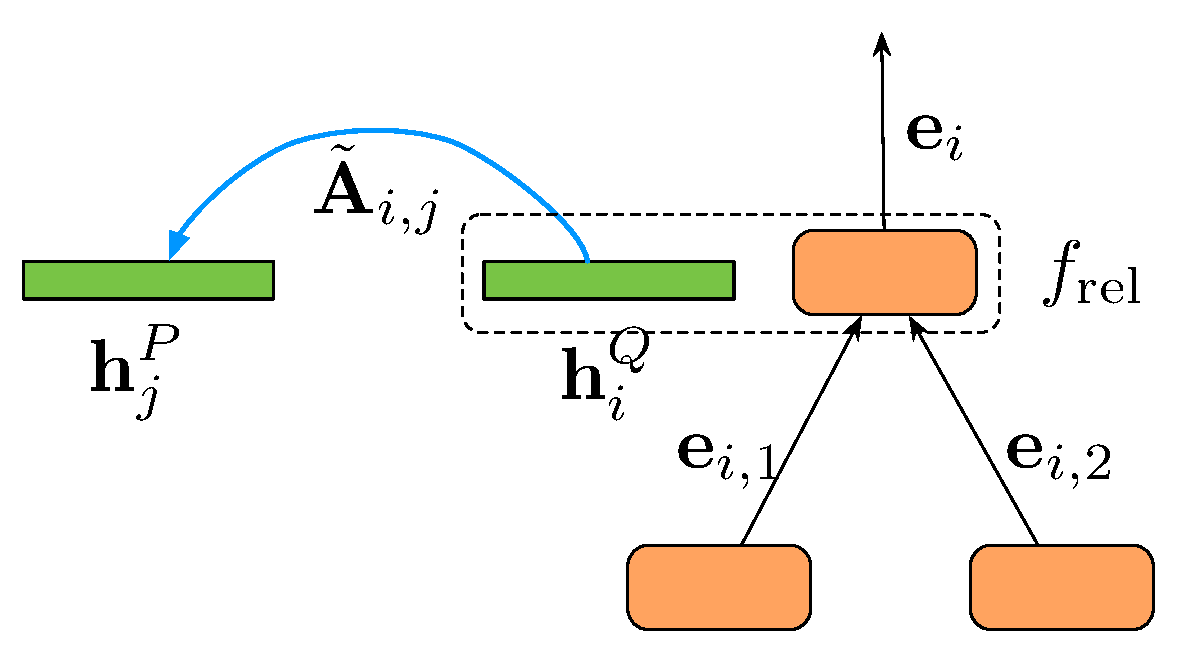
\includegraphics[width=0.65\textwidth]{entailmentlstm}
%\end{center}
\caption{Entailment composition at hypothesis tree node $i$.
The composition is based on the meaning representation
of current node $\vech_i^Q$, 
the expected alignment for node $i$, $\tilde{\mtxa}_i$,
expected meaning representation of aligned premise
tree node $\sum_{j\in P}\tilde{\mtxa}_{i,j} h_j^P$, 
and known entailment relations from children nodes 
$\vece_{i, 1}, \vece_{i,2}$.
\label{fig:entnode}
}
\end{subfigure} 
$\ $
\begin{subfigure}[b]{0.49\textwidth}
\begin{center}
$\Bigg($\raisebox{-.4\height}{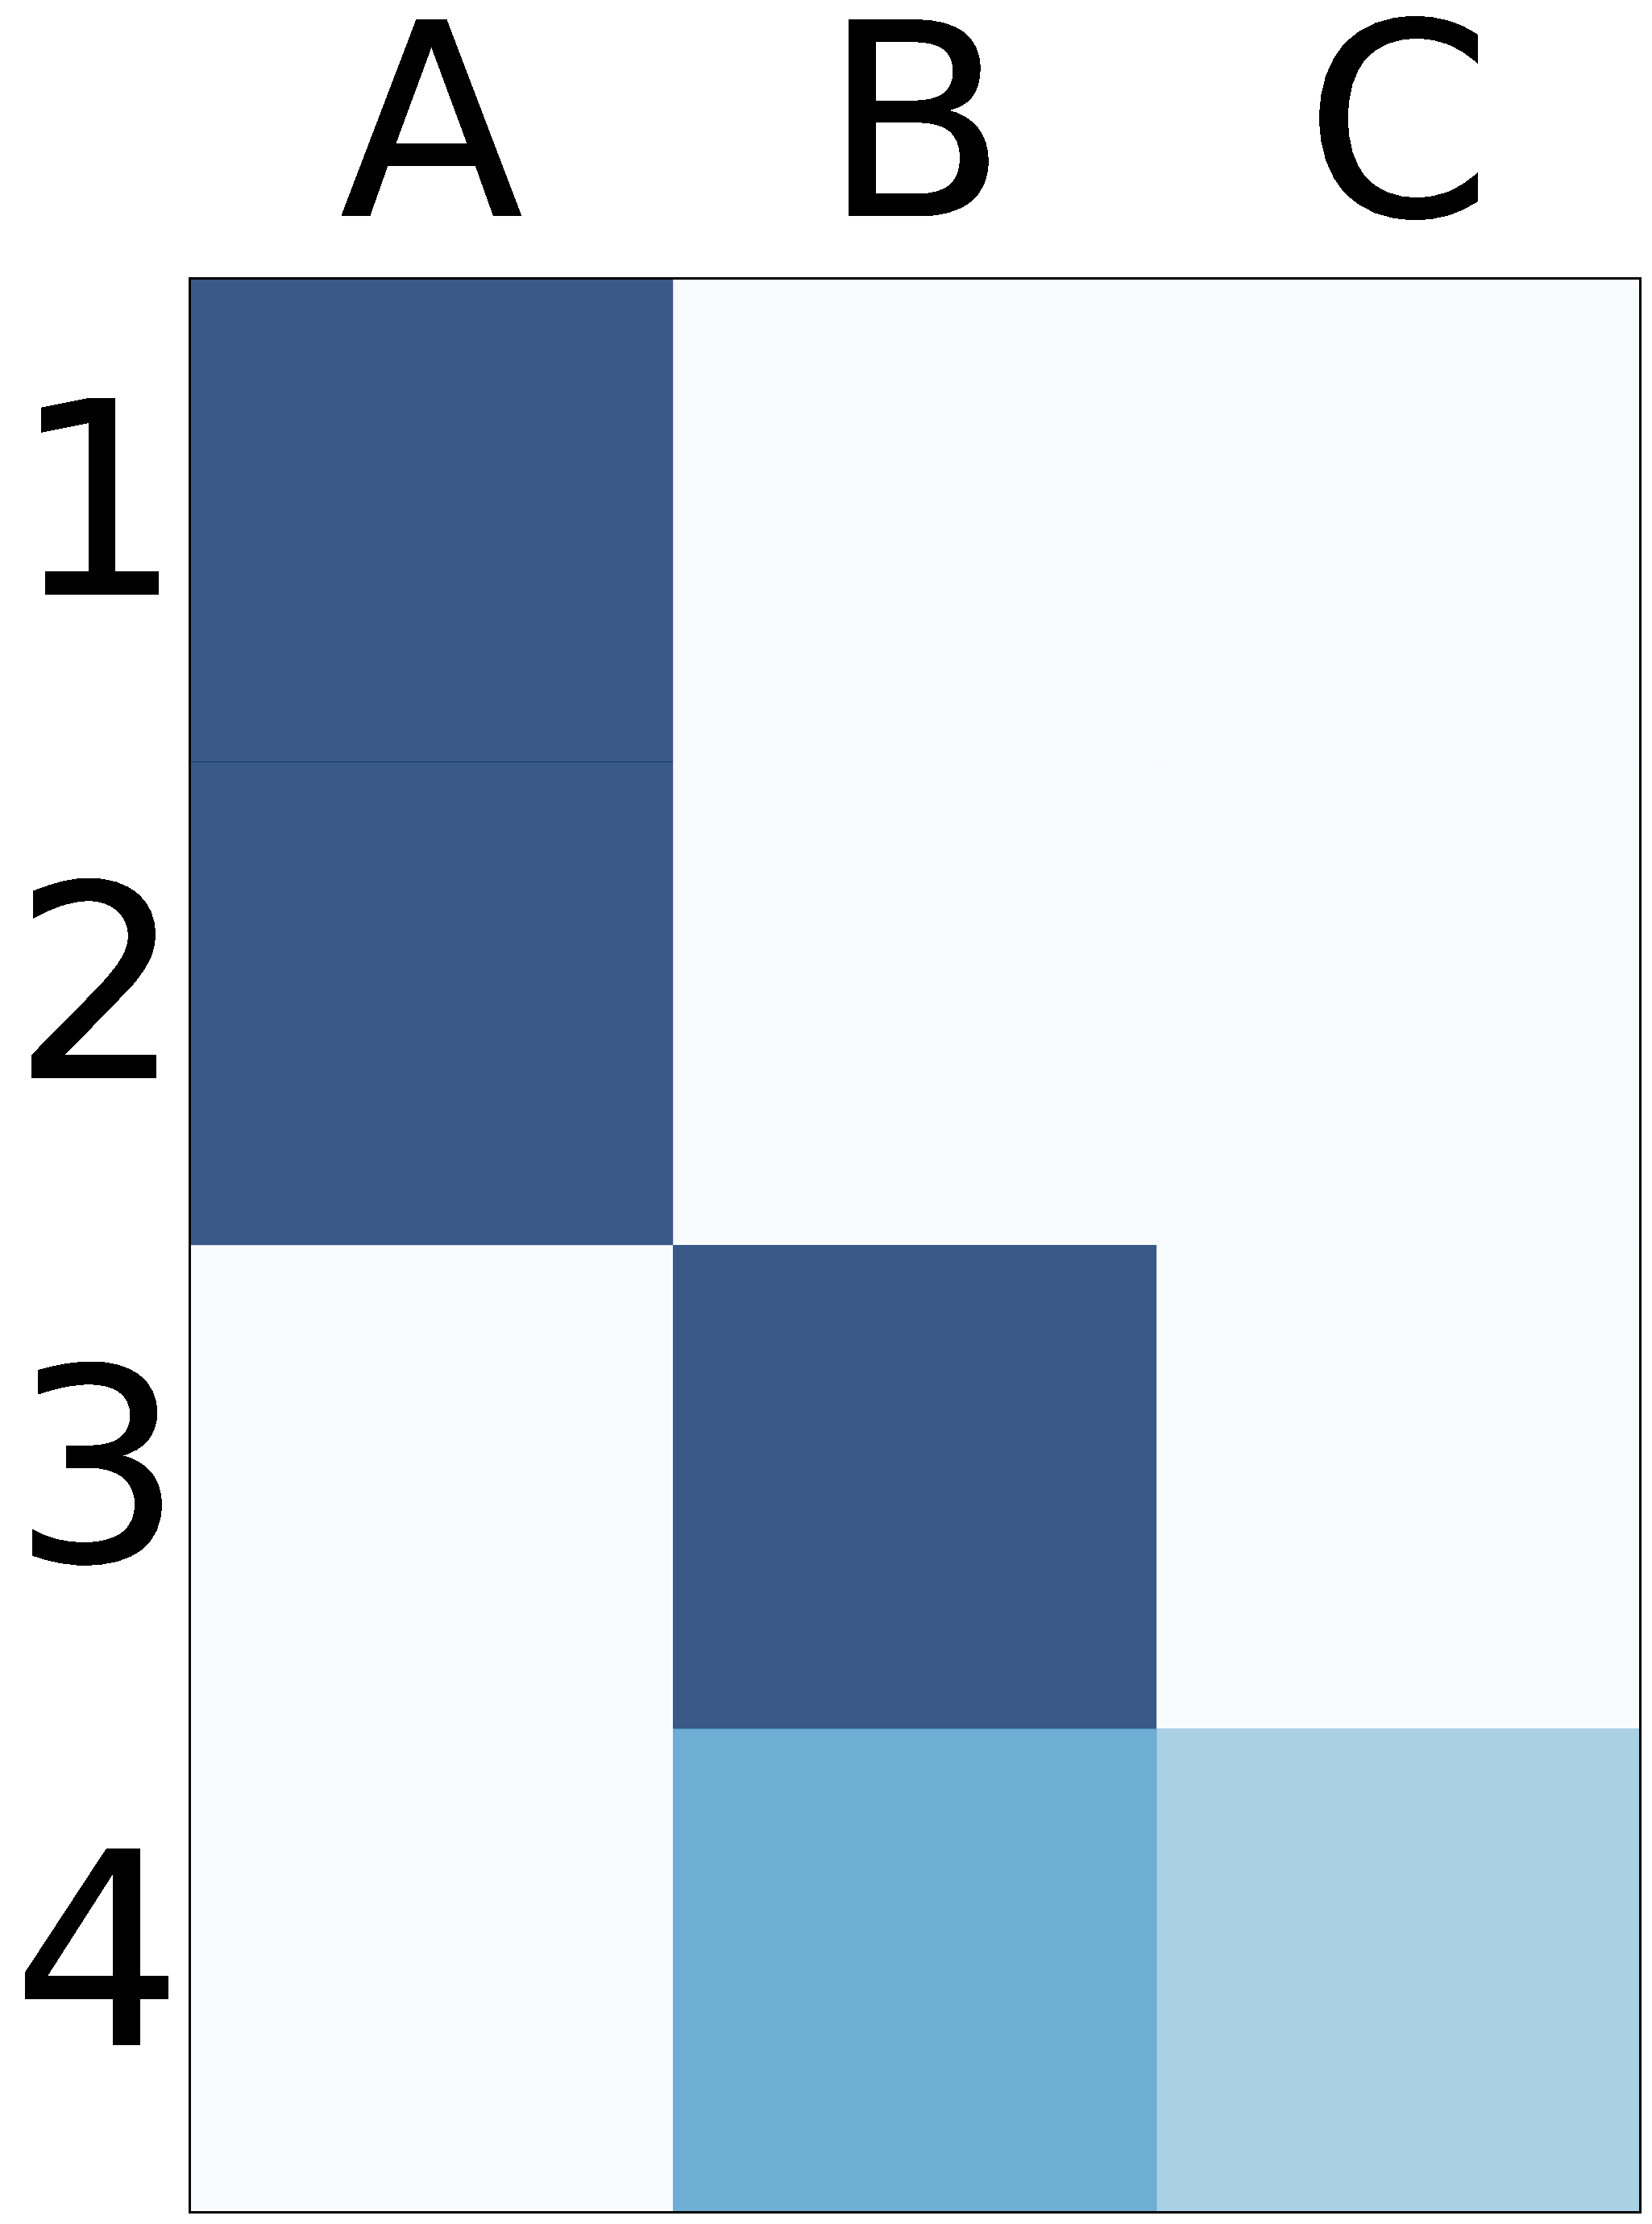
\includegraphics[width=0.16\textwidth]{dualalign.left.pdf}}$\Bigg)^{\text{T}}\quad\mathbf{\centerdot}\quad$
\raisebox{-.5\height}{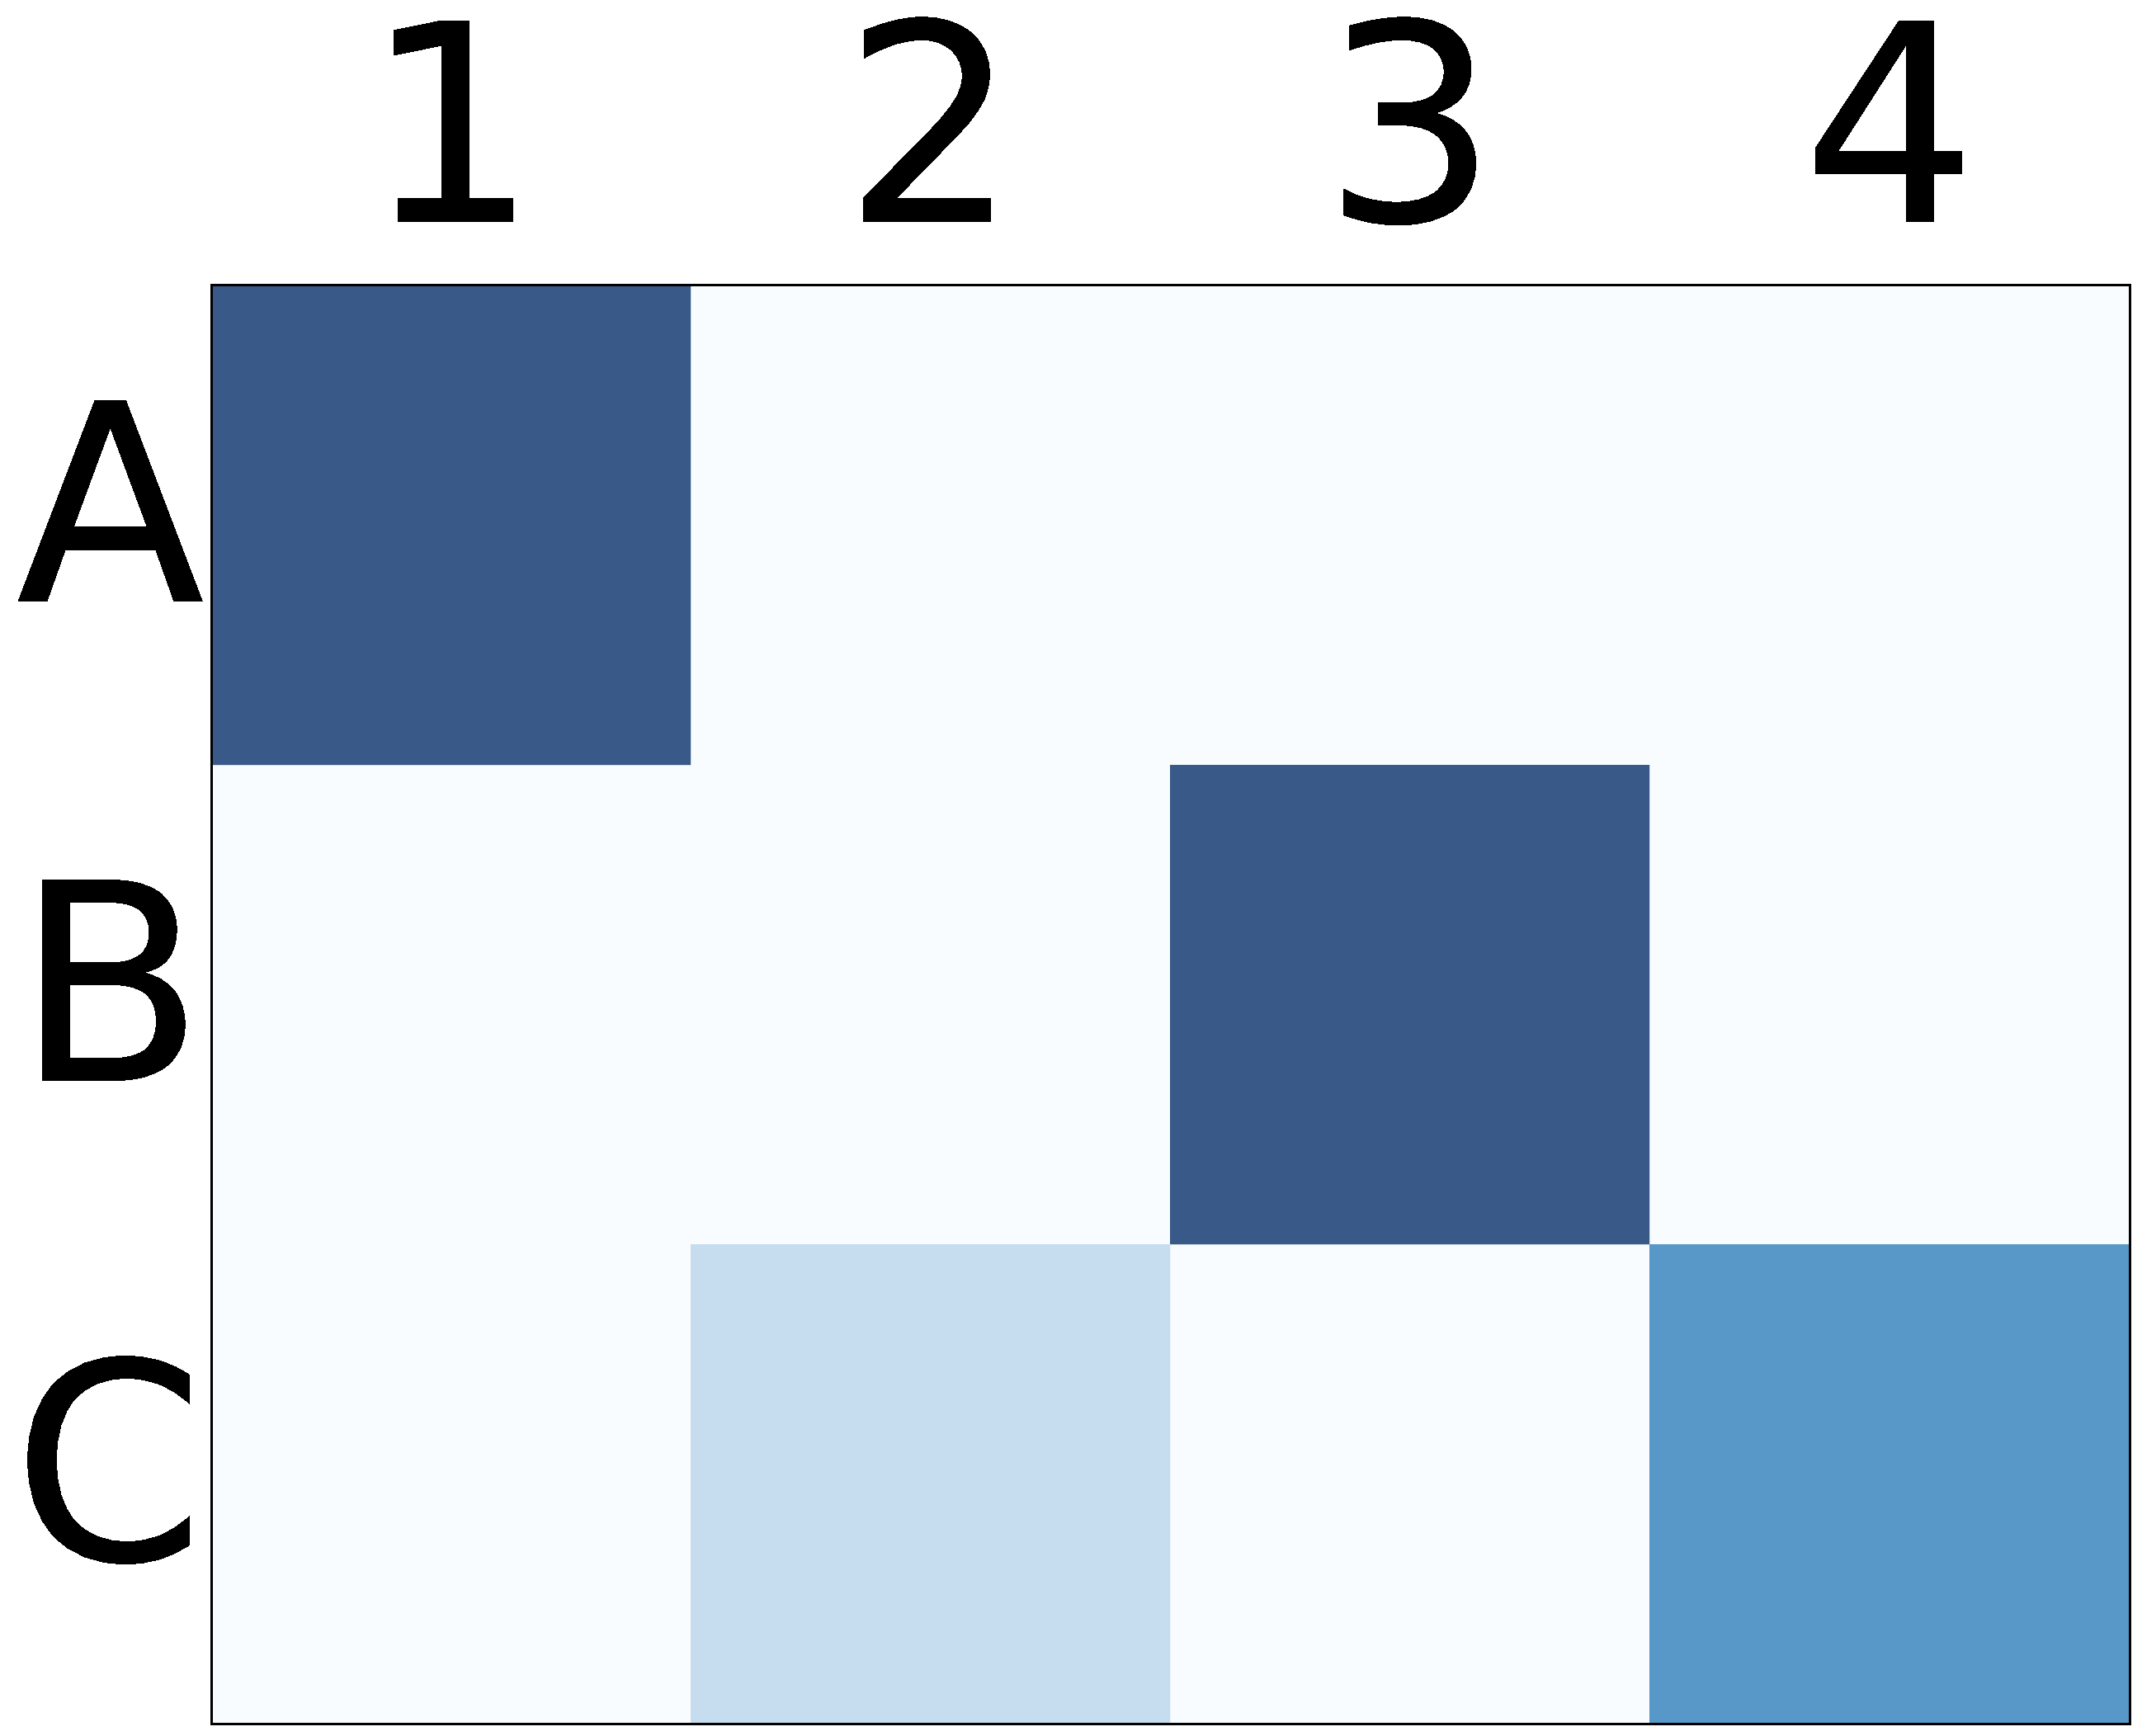
\includegraphics[width=0.2\textwidth]{dualalign.right.pdf}}$\quad=\quad$
\raisebox{-.5\height}{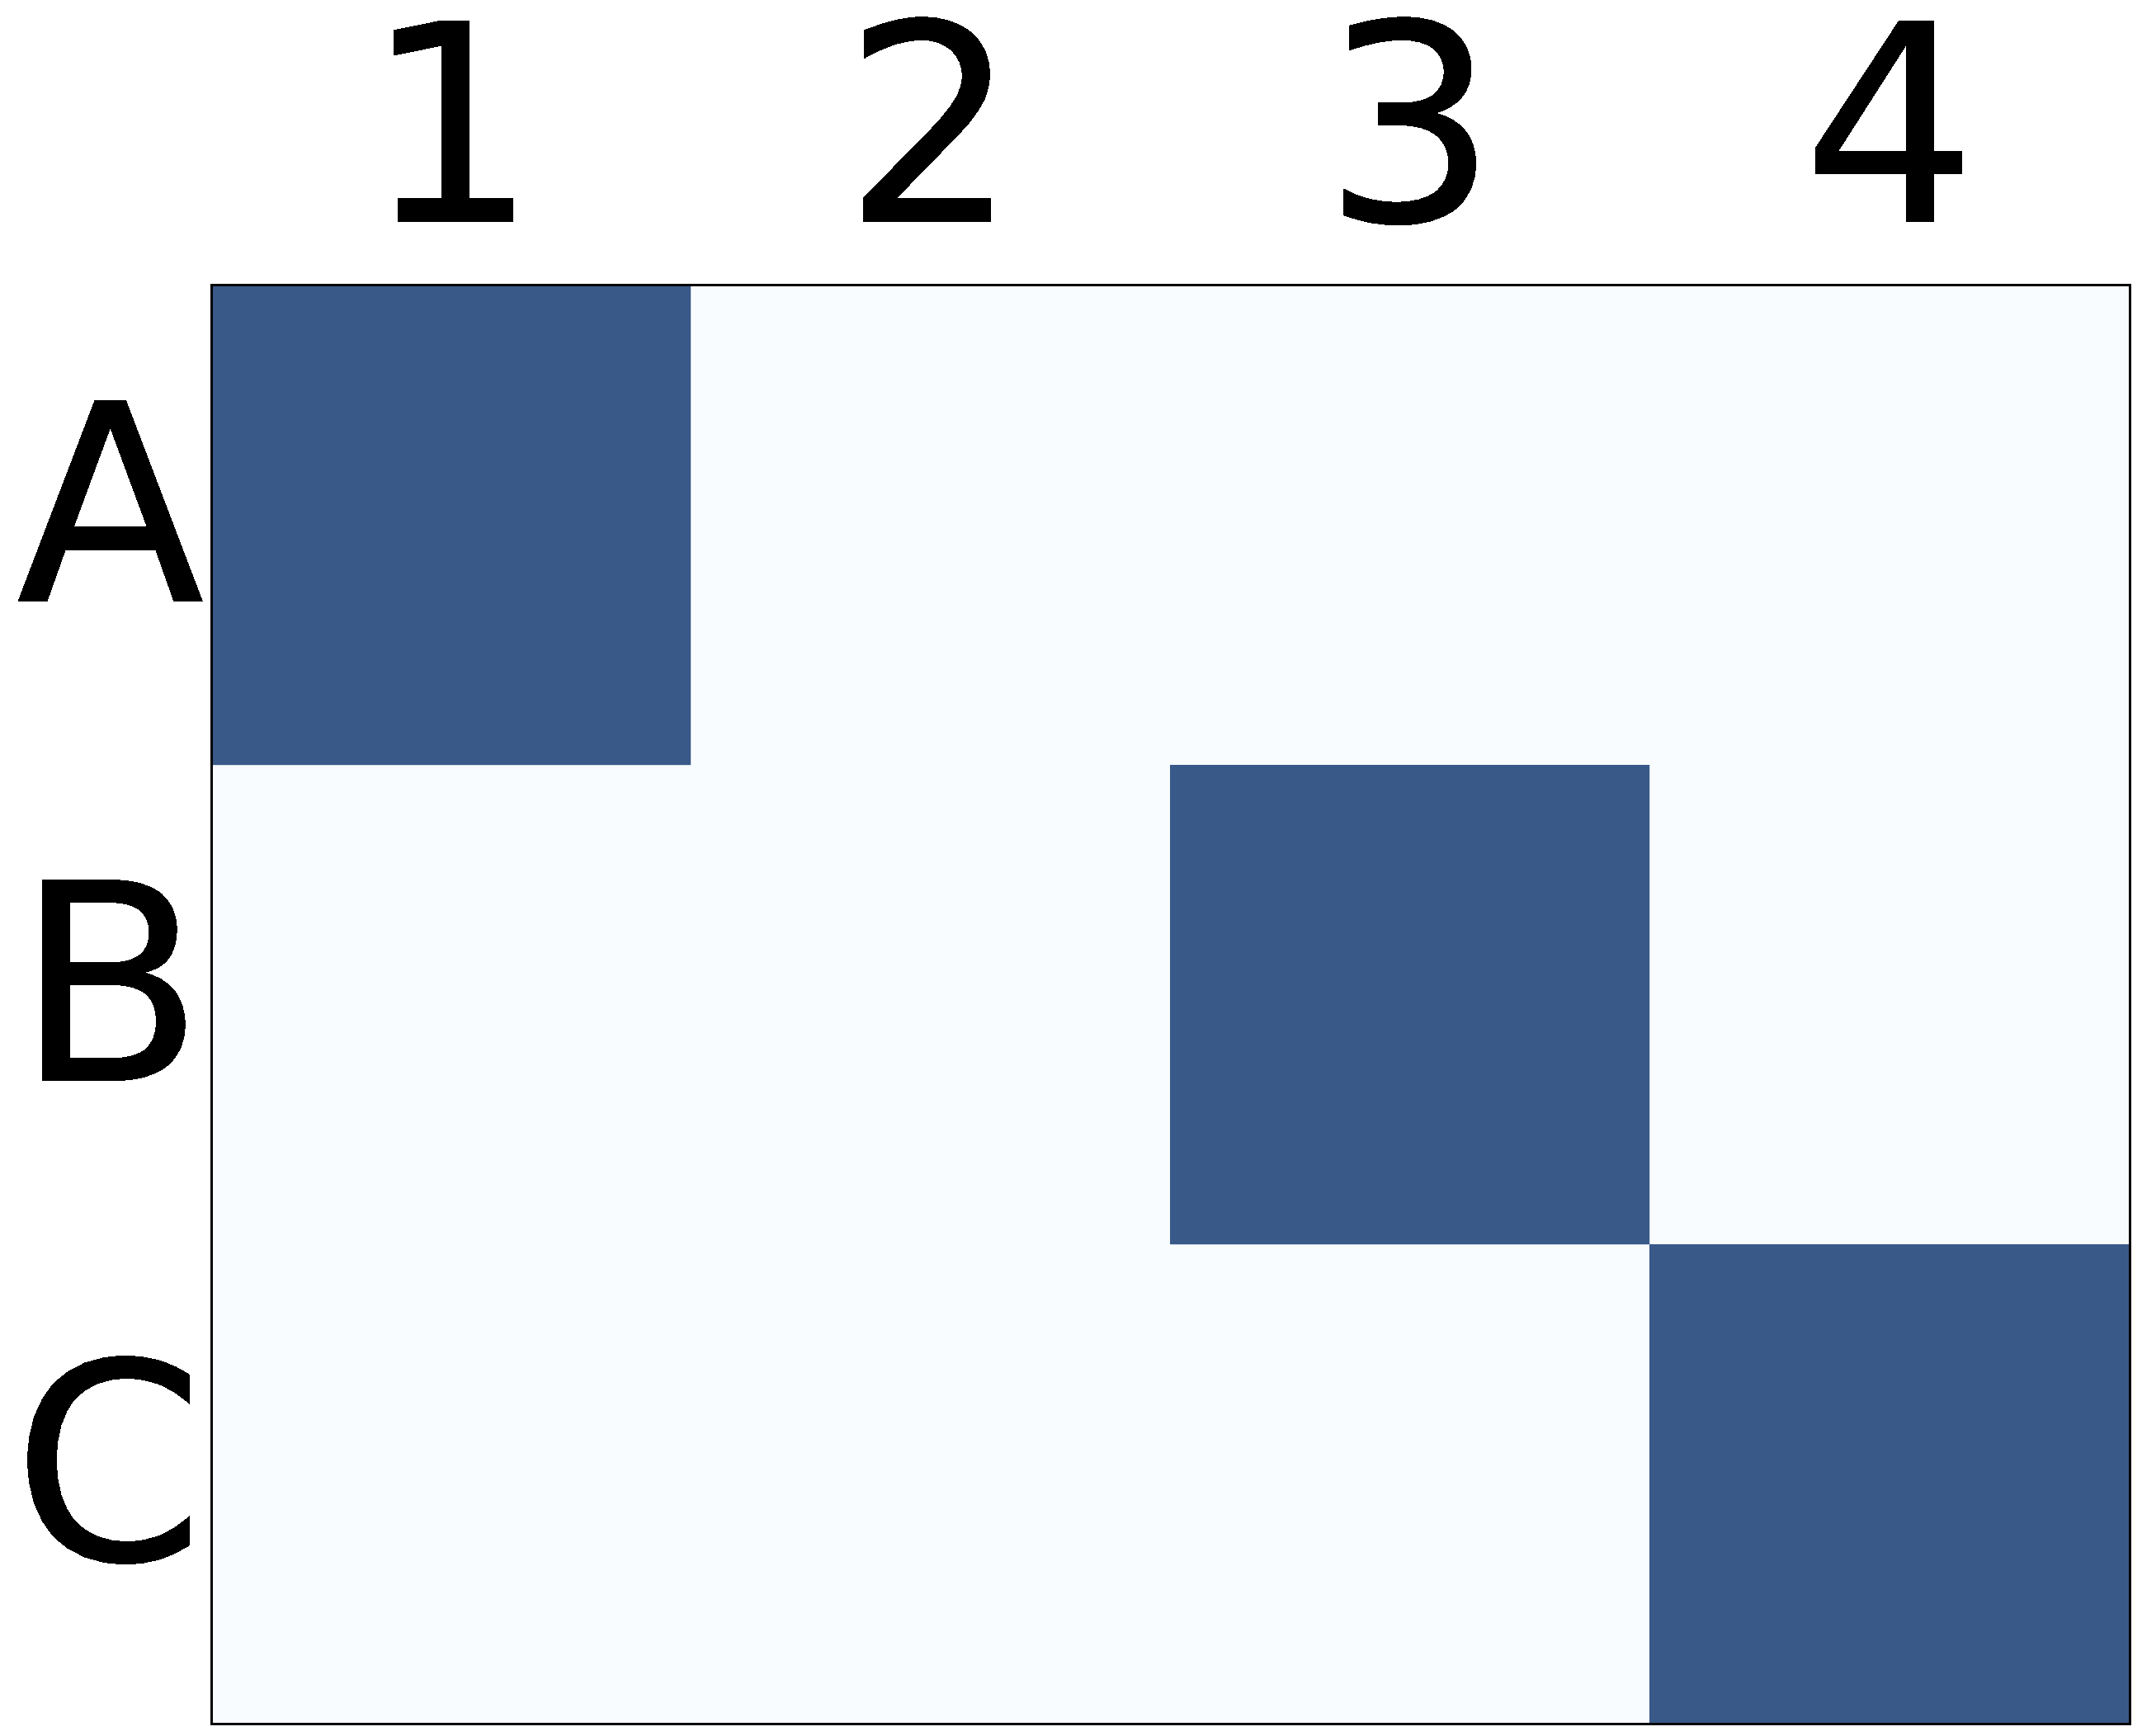
\includegraphics[width=0.2\textwidth]{dualalign.dual.pdf}}
\end{center}
\caption{An example of dual-attention eliminating
uncertainty in the alignment.
In the left attention matrix, word ``4'' can be aligned to
either ``B'' or ``C''. In the middle attention matrix,
word ``C'' can be aligned to either ``2'' or ``4''.
The element-wise product eliminates these uncertainty 
and results in the right attention matrix.
\label{fig:dualatt}
}
\end{subfigure}
\vspace{-0.4cm}
\caption{Entailment composition (a) and dual-attention calculation (b).}
\vspace{-0.5cm}
\end{figure}

\subsection{Dual-attention Over Tree Nodes}
\label{sec:dual}
\iffalse
\begin{figure}
\begin{center}
$\Bigg($\raisebox{-.4\height}{\includegraphics[width=0.08\textwidth]{figures/dualalign/left.pdf}}$\Bigg)^{\text{T}}\quad\mathbf{\centerdot}\quad$
\raisebox{-.5\height}{\includegraphics[width=0.1\textwidth]{figures/dualalign/right.pdf}}$\quad=\quad$
\raisebox{-.5\height}{\includegraphics[width=0.1\textwidth]{figures/dualalign/dual.pdf}}
\end{center}
\caption{An example of dual-attention eliminating
uncertainty in the alignment.
In the left attention matrix, word ``4'' can be aligned to
either ``B'' or ``C''. In the middle attention matrix,
word ``C'' can be aligned to either ``2'' or ``4''.
The element-wise product eliminates these uncertainty 
and results in the right attention matrix.
\label{fig:dualatt}
}
\vspace{-0.4cm}
\end{figure}
\fi

We can further improve our alignment approximation 
in Section~\ref{sec:att},
which does not consider any structural information of 
current tree, nor any alignment information from the premise
tree.

We can take a closer look at our conceptual example in 
Figure~\ref{fig:egtree}.
Note that the alignments have, to some extent, 
a symmetric property: 
if a premise node $j$ is most relevant to a hypothesis node
$i$, then the hypothesis node $i$ should also be most relevant
to premise node $j$.
For example, in Figure~\ref{fig:egtree},
the premise phrase ``hugging one another'' contradicts
the hypothesis word ``sleeping''.
In the perspective of the premise tree,
the hypothesis word ``sleeping''
contradicts by the known claim ``hugging one another''.
This suggests us to calculate the 
alignments from both side, and
eliminate the unlikely alignment
if it only exists in one side.
This technique is similar to the 
widely used forward and reversed alignment
technique in the machine translation area.

In detail, we calculate the expected alignments
$\tilde{\mtxa}$ from hypothesis to premise,
and also the expected alignments $\tilde{\mtxa}^R$
from premise to hypothesis,
and use their element-wise product
\[\tilde{\mtxa}^* = \tilde{\mtxa}\cdot\tilde{\mtxa}^R\] 
as the attention 
to feed into the Entailment Composition module.\footnote{
We need to normalize $\tilde{\mtxa}^*$ at each row to make
each row a probability distribution.
} This element-wise product is a mimic 
of the intersection %operation 
of two alignments in machine translation.
Figure~\ref{fig:dualatt} shows an example. %of dual-attention.

In addition to our dual-attention, 
\newcite{cohn2016incorporating} also explore to use the
structural information to improve the alignment.
However, their approach requires introducing 
some extra terms in the objective function, 
and is not straightforward
to integrate into our model. 
We leave adding more structural constraints
to further improve the attention 
as an open problem to explore in the future.
